\subsection {Performing Alignments}
MultiSeq can do both structural and sequence alignments.  These options
are available via the \textsf{Tools} menu in MultiSeq.

% Performing Alignments?
% detail doing both types of alignments
% maybe a para on organizing sequences into groups within sequence 
%display?

%I believe I have the majority of this subsection down, but John really ought to go over this 
\subsubsection {Structure Alignments}
MultiSeq uses the program STAMP to structurally align protein molecules.
The STAMP algorithm minimizes the $C_\alpha$ distance between aligned
residues of each molecule by applying globally optimal rigid-body
rotations and translations. Also, note that you can perform alignments
on molecules that are structurally similar. If you try to align proteins
that have no common structures, STAMP will have no means to align them.
If you would like further information about how the alignment occurs,
please refer to the STAMP manual.
\begin{figure}[here]
 \centerline{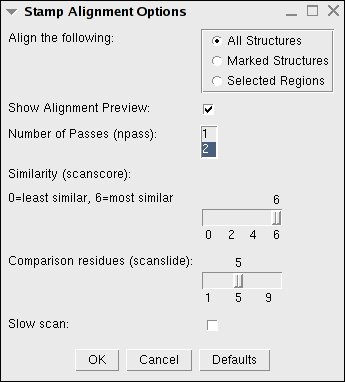
\includegraphics [width=3in]{./pictures/stamp.jpg}}
 \caption{STAMP Structural Alignment Window}%more information in caption about views etc.
 \label{stampWindow}
\end{figure}
\begin{description}     
      \item [Align the following:] Choose which structures you wish to
      align
      \item [Number of passes (npass):] Whether one or two fits are to
      be performed. The idea is that the initial fit can be used with a
      conformation biased set of parameters to improve the initial fit
      prior to fitting using distance and conformation parameters.
      Default NPASS = 1
      \item [Similarity (scanscore):] Specifies how the Sc value (STAMP
      algorithm) is to be calculated. This depends on the particular
      application. As a general rule of thumb, use SCANSCORE=6 for large
      database scans, when you are scanning with a small domain, and
      wishing to find all examples of this domain - even within large
      structures. Use SCANSCORE=1 when you wish to obtain a set of
      transformations for a set of domains which you know are similar
      (and have defined fairly precisely as domains rather than the
      larger structure that they may be a part of). Default SCANSCORE =
      6
      \item [Comparison residues (scanslide):] This is the number of
      residues that a query sequence is 'slid' along a database sequence
      to derive each initial superimposition. Initially, the N-terminus
      of the query is aligned to the 1st residue of the databse, once
      this fit has been performed and refined, and tested for good
      structural similarity, the N-terminus is aligned with the 1+th
      position, and the process repeated until the end of the database
      sequence has been reached. Default SCANSLIDE = 5
      \item [Slow scan:] If set to TRUE, then the SLOW method of getting
      the initial fits for scanning will be used (See chapter 1).
      Default SLOWSCAN = FALSE
      \item [Defaults:] resets the STAMP parameters to their original values
\end{description}


%Elijah, I'll need assistance with the description of Sequence Alignments and soon will be adding
%directions for running an alignment

\subsubsection {Sequence Alignments}

Sequence alignment in MultiSeq can be done via ClustalW or MAFFT (if you
have MAFFT locally installed) (See Fig.~\ref{seqAlignMenuWindow}).

 \begin{figure}
 \centerline{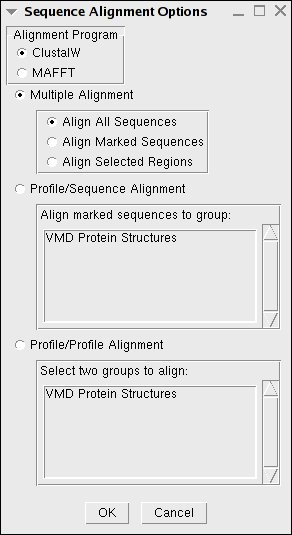
\includegraphics {./pictures/sequenceAlignmentMenu.jpg}}
 \caption{Sequence Alignment Menu Window}
\label{seqAlignMenuWindow}
\end{figure}

Once you have decided which program to use (you won't be able to select
MAFFT if you haven't configured the path to MAFFT on your local computer
via \textsf{File} | \textsf{Preferences} | \textsf{Software}), you can 
choose from 
Multiple Alignment, Profile/Sequence Alignment, or
Profile/Profile Alignment.  Once you have chosen the desired type
of alignment, you can set the proper option.

\begin{description}
     \item[Multiple Alignment]  Choose which sequences or regions you
     wish to align.
     \item[Profile/Sequence Alignment] This requires certain sequences
     to be marked, and they will then be aligned to the group that you
     specify.
     \item[Profile/Profile Alignment] To align one entire group with
     another entire group, select this option.
\end{description}

If you choose MAFFT, be aware of the following:
\begin{itemize}
\item MultiSeq has been tested with MAFFT version 6.811.  It should work
with any version of MAFFT reasonably close to that.
\item MultiSeq uses the default \textsf{-auto} option for MAFFT.
\item Profile-profile and sequence-profile alignment will be done with
MAFFT if it is chose as the desired alignment program.
\item When configuring the path to MAFFT, you need to give the path to
the `bin' directory on a unix-type system.  On Windows, give the path
that contains the `mafft.bat' file.
\end{itemize}


